\documentclass[11pt, wide, leqno]{mwart}

\usepackage{../../template}

\tit{P.1.6.}

\begin{document}
\maketitle
\tableofcontents

\section{Wstęp}\label{sec:ws}

Indiana Bill

Metoda Chudowskiego - rekord cyfr pi z 2009, na podstawie wzoru Ramanujana

\section{Pierwsze próby}
\subsection{Interpretacja geometryczna}
\label{geometric-interpretation}

Bardzo często $\pi$ jest definiowane jako stosunek obwodu okręgu do jego średnicy. W historii pojawiało się wiele prób wyznaczenia $\pi$ korzystając z obwodu wielokątów foremnych wpisanych w oraz opisanych na okręgu jednostkowym. Wraz ze wzrostem liczby boków zwiększa się dokładność oszacowań obwodu okręgu, co daje coraz to bliższe prawdy granice na wartość ludolfiny. 

Takie podejście stosował już w starożytności Archimedes. Wyprowadził on wzór rekursyjny na obwód $2n$-kąta foremnego wpisanego oraz opisanego na okręgu na podstawie obwodu $n$-kąta.

\begin{figure}[h]\centering
\begin{tikzpicture}
    \coordinate[label=left:$A_1$] (A1) at (-3, -3);
    \coordinate[label=left:$A_2$] (A2) at (-3, 3);
    \coordinate[label=right:$A_3$] (A3) at (3, 3);
    \coordinate[label=right:$A_4$] (A4) at (3, -3);

    \draw (A1)--(A2)--(A3)--(A4)--cycle;

    \coordinate[label=below:$A_1'$] (AA1) at (0, -3);
    \coordinate[label=left:$A_2'$] (AA2) at (-3, 0);
    \coordinate[label=above:$A_3'$] (AA3) at (0, 3);
    \coordinate[label=right:$A_4'$] (AA4) at (3, 0);

    \draw (AA1)--(AA2)--(AA3)--(AA4)--cycle;

    \coordinate[label=below:$B_1$] (B1) at (-1.22, -3);
    \coordinate[label=left:$B_2$] (B2) at (-3, -1.22);
    \coordinate[label=left:$B_3$] (B3) at (-3, 1.22);
    \coordinate[label=above:$B_4$] (B4) at (-1.22, 3);
    \coordinate[label=above:$B_5$] (B5) at (1.22, 3);
    \coordinate[label=right:$B_6$] (B6) at (3, 1.22);
    \coordinate[label=right:$B_7$] (B7) at (3, -1.22);
    \coordinate[label=below:$B_8$] (B8) at (1.22, -3);

    \draw (B1)--(B2)--(B3)--(B4)--(B5)--(B6)--(B7)--(B8)--cycle;
    
    \draw (3, 0)--(0, 0);
    \node at (1.5, 0.3) {$r=1$};

    \draw[very thick, ziel] (0, 0) circle (3);
    
\end{tikzpicture}
\caption{Wielokąty opisane i wpisane w okrąg o promieniu $1$.}
\label{pierwszy}
\end{figure}

Wpiszmy $n$-kąt foremny w okrąg o promieniu $1$. Teraz na tym samym okręgu opiszmy $n$-kąt tak, żeby wierzchołki wielokąta wpisanego były srodkami boków wielokąta opisywaneg. Dostajemy w ten sposob $n$-kąt foremny opisany na okręgu o promieniu $1$. Nietrudno zauważyć, że teraz jeśli połączymy sąsiednie boki $n$-kąta opisanego odcinkami styczymi do okręgu o końcach w równej odległości od najbliższego wierzchołka, to dostaniemy $2n$-kąt foremny. Sytuacja dla $n=4$ została  przedstawiona na Rysunku~\ref{pierwszy}.

Rozważmy teraz trójkąt $\Delta A_1'A_1A_2$. Zawuażmy, że odcinek $\overline{B_1B_2}$ dzieli go na dwa trójkąty podobne:
$$\Delta B_1A_1B_2\sim\Delta A_1'A_1A_2'.$$
Dla przejżystości zapisów oznaczmy $|\overline{A_1A_2}|=A$, $|\overline{B_1B_2}|=B$ oraz $|\overline{A_1'A_2'}|=a$. Z proporcji w trójkątach podobnych mamy:
\begin{align*}
    {B\over \frac12A-\frac12B}&={a\over \frac 12A}\\
    B&=\frac aA(A-B)\\
    B&=a-\frac aAB\\
    B&={aA\over A+a}
\end{align*}

Oznaczmy teraz obwód $n$-kąta wpisanego jako $l_n$, a $n$-kąta opisanego - $L_n$. Według Rysunku~\ref{pierwszy} są one równe:
\begin{align*}
    l_n&=na\\
    L_n&=nA\\
    L_{2n}&=2nB=2n{aA\over A+a}=2n^2{aA\over An+an}=2{L_nl_n\over L_n+l_n}
\end{align*}

Dalej, oznaczmy długość boku $2n$-kąta wpisanego jako $b$. Zauważmy, że wówczas:
\begin{align*}
    B&=2\tan{\pi\over 2n}\\
    a&=2\sin{\pi\over n}\\
    b&=2\sin{\pi\over 2n}
\end{align*}

oraz:
\begin{align*}
    l_{2n}&=2nb=4n\sin{\pi\over 2n}=\sqrt{16n^2\sin^2{\pi\over 2n}}=\sqrt{8n^2{\sin{\pi\over2n}\over\cos{\pi\over 2n}}2\sin{\pi\over 2n}\cos{\pi\over 2n}}=\\
    &=\sqrt{8n^2\tan{\pi\over 2n}\sin{\pi\over n}}=\sqrt{2nBna}=\sqrt{L_{2n}l_n}.
\end{align*}
\begin{figure}[!h]\centering
    \renewcommand{\figurename}{Wykres}
    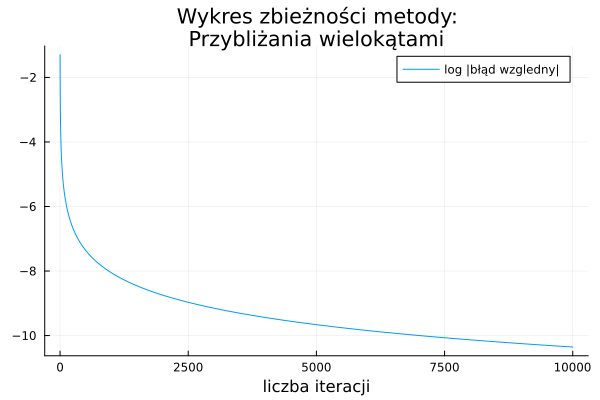
\includegraphics[width=0.6\textwidth]{../prog/geo3_log_error.png}
    \caption{Wykres logarytmu dziesiętnego z błędu względnego dla przybliżenia $\pi$ za pomocą metody geometrycznej.}
    \label{geometric-error}
\end{figure}

Zauważmy, że $\lim_{k\to\infty}L_k=2\pi$ i $\lim_{k\to\infty}l_k=2\pi$ oraz dla każdego $k$ mamy
$$l_n\leq 2\pi\leq L_n,$$
a więc możemy przybliżać $\pi$ jako
$$\pi\approx{L_n-l_n\over 4},$$
czyli jako środek przedziału $[l_n,L_n]$. Wybierzemy punkt startowy jako trójkąt równoboczny:
$$\begin{cases}
    l_3=3\sqrt3\\
    L_3=6\sqrt3
\end{cases}$$

Metoda w okolicach 8050 iteracji uzyskiwała błąd bezwzględny rzędu $10^{-12000}$. Na Wykresie~\ref{geometric-error} widzimy, że gradient wykresu logarytmu dziesiętnego od błędu względnego jest niemalże liczbą stałą. Przybliżanie liczby $\pi$ przy użyciu geometrii osiąga limit precyzji, co jest bardzo imponujące biorąc pod uwagę jak stara jest to metoda.

\begin{figure}[!h]\centering
    \renewcommand{\figurename}{Wykres}
    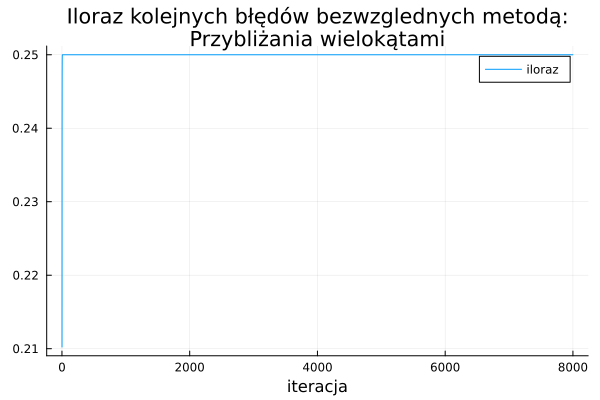
\includegraphics[width=0.7\textwidth]{../prog/geo3_error_ratio.png}
    \caption{Wykres ilorazu błędów względnych wyrazu $n+1$ i $n$ dla metody geometrycznej.}
    \label{geometric-convergence}
\end{figure}

Postawiliśmy hipotezę, że metoda ta jest zbieżna liniowo. Eksperymentalne wyznaczanie rzędu zbieżności potwierdziło to przypuszczenie, co widać na Wykresie~\ref{geometric-convergence}. Widać na nim, że
$$\lim_{n\to\infty}{|x_{n+1}-\pi|\over |x_n-\pi|}\approx\frac14,$$
gdzie $x_n$ to przybliżenie w $n$-tej iteracji.

\subsection{Algorytm Monte Carlo}

Tak jak w poprzedniej metodzie, możemy skorzystać z faktu, że dla koła jednostkowego $\pi$ jest równe jego polu. Zauważmy, że jeżeli będziemy wybierać losowo punkty kwadratu o polu 1, to $\frac\pi4$ z nich powinno znaleźć się w ćwiartce koła o środku w jednym z wierzchołków tego kwadratu (~Rysunek \ref{fig:monte-carlo}.).

\begin{figure}[!h]\centering
\begin{tikzpicture}
    \coordinate (A) at (0,0);
    \coordinate (B) at (2,0);
    \coordinate (C) at (2,2);
    \coordinate (D) at (0,2);

    \filldraw[fill=ziel!40!white, draw=ziel] (B) arc[start angle=0, end angle=90, radius=2];
    \filldraw[color=ziel!40!white] (A)--(B)--(D)--cycle;
    \draw[thick] (A)--(B)--(C)--(D)--cycle;

    \node at (0.75, 1) {\Large$\frac\pi4$};
    \node at (1, -0.3) {\large$1$};
    \node at (-0.3, 1) {\large$1$};
\end{tikzpicture}
\caption{Stosunek pola ćwiartki koła jednostkowego do kwadratu o boku $1$}
\label{fig:monte-carlo}
\end{figure}

Korzystając z algorytmu Monte Carlo możemy wybierać losowo współrzędne $x,y\in[0,1]$ kolejnych punktów, a następnie sprawdzać ile z nich spełnia warunek
$$x^2+y^2\leq1.$$
Otrzymany stosunek będzie coraz bliższy $\frac\pi4$ wraz ze zwiększaniem ilości testowanych punktów.

Na Wykresie~\ref{monte-carlo-error}. zaprezentowany jest logarytm dziesiętny z błędu względnego metody Monte Carlo. Szacowanie zbieżności tej metody wykracza poza zakres wiedzy studenta 3 semestru ze względu na losowość tego algorytmu. Wykorzystanie technik z kursu Rachunku Prawdopodobieństwa ułatwiłoby to zadanie. Na Wykresie~\ref{monte-carlo-convergence} widzimy jeden z wykresów ilorazu błędu kolejnych wyrazów jaki uzyskaliśmy przy uruchamianiu algorytmu. Na obu wykresach obserwujemy wachania lokalne zbieżności algorytmu.

\begin{figure}[!h]\centering
\renewcommand{\figurename}{Wykres}
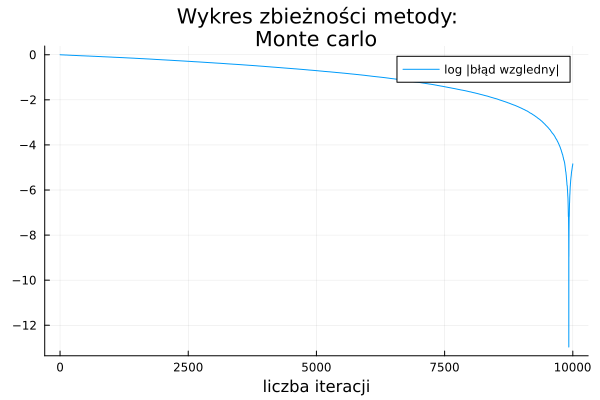
\includegraphics[width=0.6\textwidth]{../prog/monte_carlo_log_error.png}
\caption{Wykres logarytmu dziesiętnego z błędu względnego uzyskanego dla metody przybliżenia $\pi$ z pomocą algorytmu Monte Carlo.}
\label{monte-carlo-error}
\end{figure}

\begin{figure}[!h]\centering
    \renewcommand{\figurename}{Wykres}
    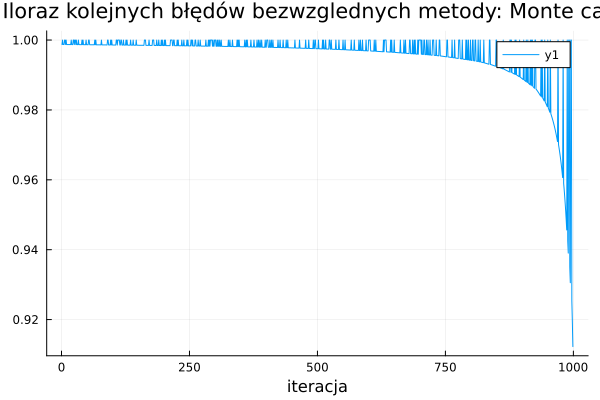
\includegraphics[width=0.6\textwidth]{../prog/monte_carlo_error_ratio.png}
    \caption{Wykres ilorazu błędów względnych wyrazu $n+1$ i $n$ dla metody z wykorzystaniem algorytmu Monte Carlo.}
    \label{monte-carlo-convergence}
\end{figure}


\subsection{Szereg Taylora}
W matematyce bardzo często w celu przybliżania porządanych wartości używa się szeregów Taylora. Tak dla przykładu, korzystając z rozszerzenia funkcji $\arctan x$ w punkcie $0$ możemy oszacować wartość $\frac\pi4$:
\begin{equation}
\begin{split}
    \frac\pi4&=\arctan1=\sum\limits_{k=0}^\infty{\arctan^{(k)}0\over k!}(1-0)^k=\\
    &=1-\frac13+\frac15-\frac17+...=\sum\limits_{k=0}^\infty{(-1)^k\over 2k+1}.
\end{split}
\end{equation}

W obliczeniach praktycznych nie możliwe jest dodawanie kolejnych elementów sumy w nieszkończoność. Konieczne jest więc zatrzymanie się na pewnym $N$, co daje pewien błąd, $R_N$:
$$\frac\pi4\approx \sum\limits_{k=0}^N{(-1)^k\over 2k+1}+R_N.$$
Oznaczmy tę sumę jako $P_N$. Ponieważ dla przybliżeń funkcji szeregiem Taylora coraz wyższego stopnia dostajemy coraz dokładniejszy wynik, to $P_{N+1}$ powinno być dokładniejsze niż $P_N$. Zauważamy też, że
$$P_{N+1}-P_N={(-1)^{N+1}\over 2N+3}$$
w takim razie możemy oszacować błąd dla szeregu Taylora $N$-tego stopnia za pomocą
$$R_N\approx \max{(-1)^{N+1}\over 2N+3}.$$

Powyższa metoda jest o wiele wolniejsza od metody Archimedesa, mimo że powstała później. W metodzie geometrycznej osiągaliśmy błąd rzędu $10^{-12000}$, natomiast wzór Taylora daje błąd rzędu $10^{-10}$. Iloraz wyrazu $n+1$ do wyrazu $n$ eksperymentalnie zbiega do 1, co sugeruje zbieżność nadliniową \cite{bog}.

\begin{figure}[!h]\centering
    \renewcommand{\figurename}{Wykres}
    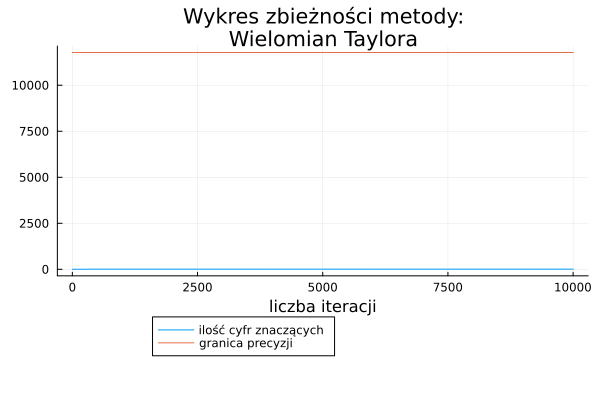
\includegraphics[width=0.7\textwidth]{../prog/taylor_log_error.png}
    \caption{Wykres logarytmu dziesiętnego z błędu względnego uzyskanego dla metody przybliżenia $\pi$ za pomocą szeregu Taylora.}
    \label{taylor-series-error}
\end{figure}

\begin{figure}[!h]\centering
    \renewcommand{\figurename}{Wykres}
    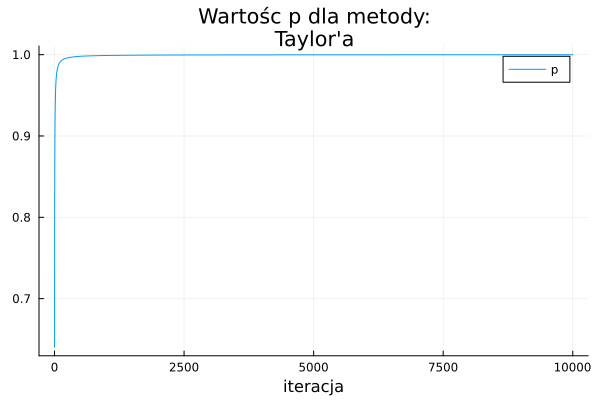
\includegraphics[width=0.7\textwidth]{../prog/taylor_error_ratio.png}
    \caption{Wykres ilorazu błędów względnych wyrazu $n+1$ i $n$ dla metody z wykorzystaniem szeregu Taylora.}
    \label{taylor-series-convergence}
\end{figure}




\section{Wzór Viete'a}

% https://en.wikipedia.org/wiki/Vi%C3%A8te%27s_formula

$$\pi=\lim\limits_{k\to\infty}2^k\sqrt{2-a_k}$$
$$a_1=0$$
$$a_k=\sqrt{2+a_{k+1}}$$

\section{Algorytm Chudnowsky'ch}

Algorytm zaproponowany przez braci Chudnowskych opiera się na 17 wzorach na $\frac1\pi$ opracowanych przez Srinivasa Ramanujan\cite{review}:
$${\frac {1}{\pi }}={\frac {1}{426880{\sqrt {10005}}}}\sum _{k=0}^{\infty }{\frac {(6k)!(13591409+545140134k)}{(3k)!(k!)^{3}(-640320)^{3k}}}.$$
Z tego można uzyskać $\pi$ wprost w formie wzoru:
$$\pi=C\Big(\sum\limits_{q=0}^\infty{M_q\cdot L_q\over X_q}\Big)^{-1},$$
gdzie 
$$
\begin{cases}
    C=426880\sqrt{10005}\\
    L_{q+1}=L_q+545140134 \quad L_0=13591409  \\
    X_{q+1}=X_q\cdot(-262537412640768000)\quad X_0=1\\
    K_{q+1}=K_q+12\quad K_0=-6\\
    M_{q+1}=M_{q}\cdot \left({\frac {K_{q+1}^{3}-16K_{q+1}}{\left(q+1\right)^{3}}}\right)\quad M_{0}=1.
\end{cases}
$$
Aby wyprowadzić ten wzór, jak i inne podane przez Ramanujana, potrzebna jest znajomość między innymi teorii funkcji eliptycznych\cite{review}. Z tego też względu w tym reporcie nie podejmiemy się uzasadniania poprawności wyżej podanego wzoru. Dla zainteresowanych polecamy lekturę "Collected Papers of Srinivasa Ramanujan"\cite{ramanujan}.

\begin{figure}[!h]
    \centering
    \renewcommand{\figurename}{Wykres}
    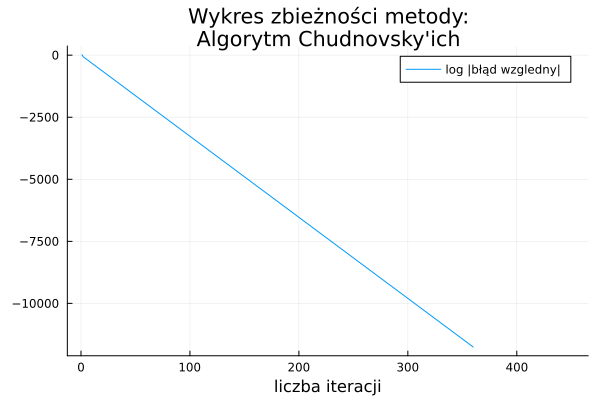
\includegraphics[width=0.6\textwidth]{../prog/chudnowsky_log_error.png}
    \caption{Wykres ilości cyfr znaczących uzyskanych dla  przybliżenia  $\pi$ za pomocą algorytmu braci Chudnowskych.}
    \label{chudnowsky-error}
\end{figure}

\begin{figure}[!h]
    \centering
    \renewcommand{\figurename}{Wykres}
    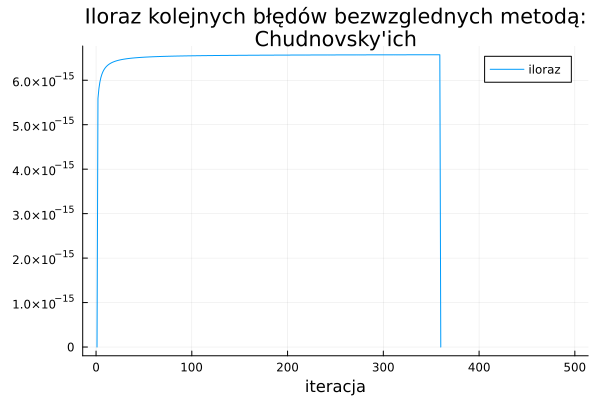
\includegraphics[width=0.6\textwidth]{../prog/chudnowsky_error_ratio.png}
    \caption{Wykres estymowanej wartości p dla algorytmu Chudowskych.}
    \label{chudnowsky-convergence}
\end{figure}

\subsection{Wyniki}

Liczba dokładnie wyznaczonych cyfr, w zależności od liczby iteracji została zaprezentowana na Wykresie~\ref{chudnowsky-error}. Już dla 359 iteracji błąd bezwzględny jest równy 0. Każe to sugerować, że to właśnie ta metoda została użyta jako implementacja funkcji \verb+pi()+ w języku \verb+Julia+. Powoduje to anomalie widoczne na wykresach.

Eksperymentalne wyznaczanie zbieżności metody Chudnowskych sugeruje zbieżność liniowa, tak jak na Wykresie~\ref{chudnowsky-convergence}.. Nietypowe załamanie w okolicach 359 iteracji jest spowodowane zerową wartością błędu bezwzględnego w tym miejscu. Z pozostałej części wykresu możemy wydedukować, że
$$\lim_{k\to\infty}{{|x_{k+1}-\pi|\over |x_k-\pi|}}\approx 6.5\cdot 10^{-15},$$
gdzie $x_k$ to oszacowanie $\pi$ uzyskane w $k$-tej iteracji.
% https://www.maa.org/sites/default/files/pdf/pubs/amm_supplements/Monthly_Reference_5.pdf

\section{Algorytm Gaussa-Legendre'a}

Algorytm Gaussa-Legendre'a jest aktualnie jednym z najszybciej zbiegających algorytmów używanych do wyliczania liczb $\pi$. Został wyprowadzony na podstawie prac Carla Friedricha Gaussa oraz Adrien-Marie Legendre na podstawie współczesnych algorytmów do mnożenia i pierwiastkowania.Jest on, niestety, bardzo wymagający pamięciowo. Poniżej prezentujemy implementację tego algorytmu\cite{gausse2}:

\newpage

\begin{lstlisting}[language=ps]
function gauss_legrendre (max):
    a = 1
    b = 1 / sqrt(2)
    t = 1 / 4
    p = 1
    i = 0
    while i <= max:
        an = (a + b) / 2
        b = sqrt(a * b)
        t = t - p * (a - an) * (a - an)
        p = 2 * p
        a = an
    
    return (a + b) * (a + b) / (4 * t)
\end{lstlisting}

\subsection{Wyniki}

Metoda Gaussa-Legrendre'a okazała się zbiegać do implementacji bibliotecznej funkcji \verb+pi()+ z języka \verb+Julia+ wyjątkowo szybko, bo już w 11 iteracji kwadrat błędu maszynowo był równy zeru, co widać na Wykresie~\ref{gauss-error}.

\begin{figure}[!h]
    \centering
    \renewcommand{\figurename}{Wykres}
    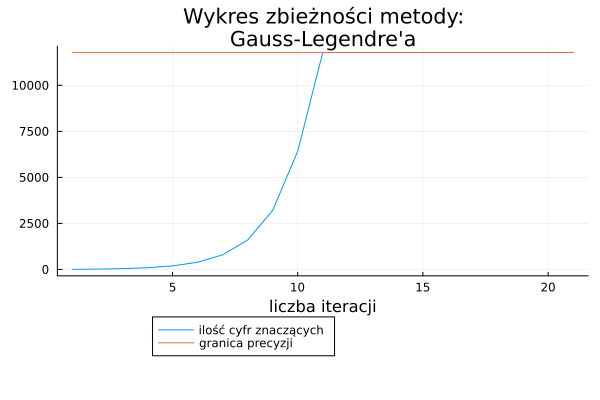
\includegraphics[width=0.7\textwidth]{../prog/gauss_legendre_log_error.png}
    \caption{Wykres logarytmu dziesiętnego z błędu względnego dla przybliżenia $\pi$ za pomocą algorytmu Gaussa-Legendre'a.}
    \label{gauss-error}
\end{figure}

\begin{figure}[!h]
    \centering
    \renewcommand{\figurename}{Wykres}
    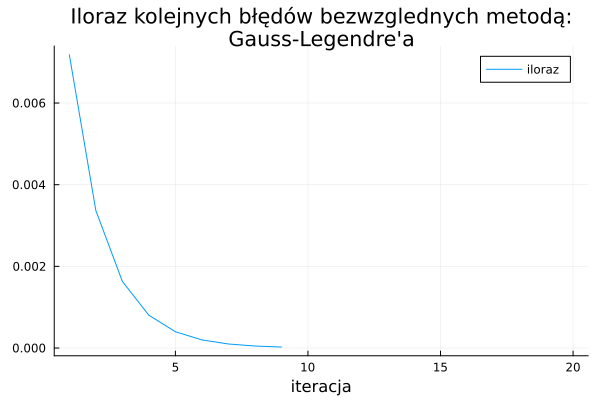
\includegraphics[width=0.7\textwidth]{../prog/gauss_legendre_error_ratio.png}
    \caption{Wykres ilorazu błędów względnych wyrazu $n+1$ i $n$ dla algorytmu Gaussa-Legrendre'a.}
    \label{gauss-convergence}
\end{figure}

Eksperymentalne obliczenia rzędu zbieżności tej metody jedynie potwierdzają wyższą zbieżność tego algorytmu niż w przypadku innych opisanych metod (Wykres~\ref{gauss-convergence}). Dla precyzji wynoszącej 16 069 bitów obliczenia na podstawie dzielenia błędu $(n+1)$-ego wyrazu przez kwadrat błędu $n$-tego wyrazu nie dają konkretnych wyników przez zbyt szybkie dążenie tej metody do $\pi$. W literaturze metoda ta jest określana jako zbieżna kwadratowo \cite{gausse-smth}.

Pomimo tak dobrej zbieżności, metoda ta nie jest powszechnie wykorzystywana, gdyż zużywa więcej pamięci niż metoda Chudnowskych.

\newpage

Wartość $\pi$ obliczona dla 10 iteracji naszego programu daje:

{\scriptsize
3.14159265358979323846264338327950288419716939937510582097494459230781640628620899862803482534211706798214808651\\
32823066470938446095505822317253594081284811174502841027019385211055596446229489549303819644288109756659334461284756\\
4823378678316527120190914564856692346034861045432664821339360726024914127372458700660631558817488152092096282925409\\
171536436789259036001133053054882046652138414695194151160943305727036575959195309218611738193261179310511854807446\\
2379962749567351885752724891227938183011949129833673362440656643086021394946395224737190702179860943702770539217176\\
2931767523846748184676694051320005681271452635608277857713427577896091736371787214684409012249534301465495853710507\\
9227968925892354201995611212902196086403441815981362977477130996051870721134999999837297804995105973173281609631859\\
50244594553469083026425223082533446850352619311881710100031378387528865875332083814206171776691473035982534904287554\\
68731159562863882353787593751957781857780532171226806613001927876611195909216420198938095257201065485863278865936153\\
38182796823030195203530185296899577362259941389124972177528347913151557485724245415069595082953311686172785588907509\\
83817546374649393192550604009277016711390098488240128583616035637076601047101819429555961989467678374494482553797747\\
26847104047534646208046684259069491293313677028989152104752162056966024058038150193511253382430035587640247496473263\\
91419927260426992279678235478163600934172164121992458631503028618297455570674983850549458858692699569092721079750930\\
29553211653449872027559602364806654991198818347977535663698074265425278625518184175746728909777727938000816470600161\\
45249192173217214772350141441973568548161361157352552133475741849468438523323907394143334547762416862518983569485562\\
09921922218427255025425688767179049460165346680498862723279178608578438382796797668145410095388378636095068006422512\\
52051173929848960841284886269456042419652850222106611863067442786220391949450471237137869609563643719172874677646575\\
73962413890865832645995813390478027590099465764078951269468398352595709825822620522489407726719478268482601476990902\\
64013639443745530506820349625245174939965143142980919065925093722169646151570985838741059788595977297549893016175392\\
84681382686838689427741559918559252459539594310499725246808459872736446958486538367362226260991246080512438843904512\\
44136549762780797715691435997700129616089441694868555848406353422072225828488648158456028506016842739452267467678895\\
25213852254995466672782398645659611635488623057745649803559363456817432411251507606947945109659609402522887971089314\\
566913686722874894056010150330861792868092087476091782493858900971490967598526136554978189312978482168299894872...
}

\end{document}